\documentclass[twoside]{book}

% Packages required by doxygen
\usepackage{fixltx2e}
\usepackage{calc}
\usepackage{doxygen}
\usepackage[export]{adjustbox} % also loads graphicx
\usepackage{graphicx}
\usepackage[utf8]{inputenc}
\usepackage{makeidx}
\usepackage{multicol}
\usepackage{multirow}
\PassOptionsToPackage{warn}{textcomp}
\usepackage{textcomp}
\usepackage[nointegrals]{wasysym}
\usepackage[table]{xcolor}

% Font selection
\usepackage[T1]{fontenc}
\usepackage[scaled=.90]{helvet}
\usepackage{courier}
\usepackage{amssymb}
\usepackage{sectsty}
\renewcommand{\familydefault}{\sfdefault}
\allsectionsfont{%
  \fontseries{bc}\selectfont%
  \color{darkgray}%
}
\renewcommand{\DoxyLabelFont}{%
  \fontseries{bc}\selectfont%
  \color{darkgray}%
}
\newcommand{\+}{\discretionary{\mbox{\scriptsize$\hookleftarrow$}}{}{}}

% Page & text layout
\usepackage{geometry}
\geometry{%
  a4paper,%
  top=2.5cm,%
  bottom=2.5cm,%
  left=2.5cm,%
  right=2.5cm%
}
\tolerance=750
\hfuzz=15pt
\hbadness=750
\setlength{\emergencystretch}{15pt}
\setlength{\parindent}{0cm}
\setlength{\parskip}{3ex plus 2ex minus 2ex}
\makeatletter
\renewcommand{\paragraph}{%
  \@startsection{paragraph}{4}{0ex}{-1.0ex}{1.0ex}{%
    \normalfont\normalsize\bfseries\SS@parafont%
  }%
}
\renewcommand{\subparagraph}{%
  \@startsection{subparagraph}{5}{0ex}{-1.0ex}{1.0ex}{%
    \normalfont\normalsize\bfseries\SS@subparafont%
  }%
}
\makeatother

% Headers & footers
\usepackage{fancyhdr}
\pagestyle{fancyplain}
\fancyhead[LE]{\fancyplain{}{\bfseries\thepage}}
\fancyhead[CE]{\fancyplain{}{}}
\fancyhead[RE]{\fancyplain{}{\bfseries\leftmark}}
\fancyhead[LO]{\fancyplain{}{\bfseries\rightmark}}
\fancyhead[CO]{\fancyplain{}{}}
\fancyhead[RO]{\fancyplain{}{\bfseries\thepage}}
\fancyfoot[LE]{\fancyplain{}{}}
\fancyfoot[CE]{\fancyplain{}{}}
\fancyfoot[RE]{\fancyplain{}{\bfseries\scriptsize Generated by Doxygen }}
\fancyfoot[LO]{\fancyplain{}{\bfseries\scriptsize Generated by Doxygen }}
\fancyfoot[CO]{\fancyplain{}{}}
\fancyfoot[RO]{\fancyplain{}{}}
\renewcommand{\footrulewidth}{0.4pt}
\renewcommand{\chaptermark}[1]{%
  \markboth{#1}{}%
}
\renewcommand{\sectionmark}[1]{%
  \markright{\thesection\ #1}%
}

% Indices & bibliography
\usepackage{natbib}
\usepackage[titles]{tocloft}
\setcounter{tocdepth}{3}
\setcounter{secnumdepth}{5}
\makeindex

% Hyperlinks (required, but should be loaded last)
\usepackage{ifpdf}
\ifpdf
  \usepackage[pdftex,pagebackref=true]{hyperref}
\else
  \usepackage[ps2pdf,pagebackref=true]{hyperref}
\fi
\hypersetup{%
  colorlinks=true,%
  linkcolor=blue,%
  citecolor=blue,%
  unicode%
}

% Custom commands
\newcommand{\clearemptydoublepage}{%
  \newpage{\pagestyle{empty}\cleardoublepage}%
}

\usepackage{caption}
\captionsetup{labelsep=space,justification=centering,font={bf},singlelinecheck=off,skip=4pt,position=top}

%===== C O N T E N T S =====

\begin{document}

% Titlepage & ToC
\hypersetup{pageanchor=false,
             bookmarksnumbered=true,
             pdfencoding=unicode
            }
\pagenumbering{roman}
\begin{titlepage}
\vspace*{7cm}
\begin{center}%
{\Large My Project }\\
\vspace*{1cm}
{\large Generated by Doxygen 1.8.11}\\
\end{center}
\end{titlepage}
\clearemptydoublepage
\tableofcontents
\clearemptydoublepage
\pagenumbering{arabic}
\hypersetup{pageanchor=true}

%--- Begin generated contents ---
\chapter{Class Index}
\section{Class List}
Here are the classes, structs, unions and interfaces with brief descriptions\+:\begin{DoxyCompactList}
\item\contentsline{section}{\hyperlink{classBoy}{Boy} }{\pageref{classBoy}}{}
\item\contentsline{section}{\hyperlink{classcouple}{couple} }{\pageref{classcouple}}{}
\item\contentsline{section}{\hyperlink{classGift}{Gift} }{\pageref{classGift}}{}
\item\contentsline{section}{\hyperlink{classGirl}{Girl} }{\pageref{classGirl}}{}
\end{DoxyCompactList}

\chapter{File Index}
\section{File List}
Here is a list of all files with brief descriptions\+:\begin{DoxyCompactList}
\item\contentsline{section}{\hyperlink{boy_8cpp}{boy.\+cpp} }{\pageref{boy_8cpp}}{}
\item\contentsline{section}{\hyperlink{boy_8h}{boy.\+h} }{\pageref{boy_8h}}{}
\item\contentsline{section}{\hyperlink{couple_8cpp}{couple.\+cpp} }{\pageref{couple_8cpp}}{}
\item\contentsline{section}{\hyperlink{couple_8h}{couple.\+h} }{\pageref{couple_8h}}{}
\item\contentsline{section}{\hyperlink{gift_8cpp}{gift.\+cpp} }{\pageref{gift_8cpp}}{}
\item\contentsline{section}{\hyperlink{gift_8h}{gift.\+h} }{\pageref{gift_8h}}{}
\item\contentsline{section}{\hyperlink{girl_8cpp}{girl.\+cpp} }{\pageref{girl_8cpp}}{}
\item\contentsline{section}{\hyperlink{girl_8h}{girl.\+h} }{\pageref{girl_8h}}{}
\item\contentsline{section}{\hyperlink{Q1_8cpp}{Q1.\+cpp} }{\pageref{Q1_8cpp}}{}
\item\contentsline{section}{\hyperlink{Q2_8cpp}{Q2.\+cpp} }{\pageref{Q2_8cpp}}{}
\end{DoxyCompactList}

\chapter{Class Documentation}
\hypertarget{classBoy}{}\section{Boy Class Reference}
\label{classBoy}\index{Boy@{Boy}}


{\ttfamily \#include $<$boy.\+h$>$}

\subsection*{Public Member Functions}
\begin{DoxyCompactItemize}
\item 
void \hyperlink{classBoy_aa6d16a472a01b4e7da0817fe94d9a2bd}{init} (std\+::string boyname, std\+::string boytype, int boyattr, int boyintelli, int boybud)
\item 
int \hyperlink{classBoy_a72ac2c3f82b5dbd6ec97bf46dfd62681}{get\+Status} ()
\item 
void \hyperlink{classBoy_a2a8cc82d9332c07eb475198e46028d52}{change\+Status} ()
\item 
void \hyperlink{classBoy_a1ffc629e12e8a14b48c5b65133af9809}{change\+Budget} (int price)
\item 
int \hyperlink{classBoy_a05c48b12091ebcad44ba86ba88514ac5}{get\+Budget} ()
\item 
int \hyperlink{classBoy_adb7888ec543c4dcba1bcb1d7e32d7ed1}{get\+Intelli} ()
\item 
int \hyperlink{classBoy_a555fc2dfb930f29fdc384f5d7013759b}{get\+Attr} ()
\item 
std\+::string \hyperlink{classBoy_acf59fd0074a6ea3413751a95b2970303}{get\+Name} ()
\item 
std\+::string \hyperlink{classBoy_a04fcc2f16f9e3d569c64d23a73d9e258}{get\+Type} ()
\end{DoxyCompactItemize}


\subsection{Member Function Documentation}
\index{Boy@{Boy}!change\+Budget@{change\+Budget}}
\index{change\+Budget@{change\+Budget}!Boy@{Boy}}
\subsubsection[{\texorpdfstring{change\+Budget(int price)}{changeBudget(int price)}}]{\setlength{\rightskip}{0pt plus 5cm}void Boy\+::change\+Budget (
\begin{DoxyParamCaption}
\item[{int}]{price}
\end{DoxyParamCaption}
)}\hypertarget{classBoy_a1ffc629e12e8a14b48c5b65133af9809}{}\label{classBoy_a1ffc629e12e8a14b48c5b65133af9809}
\index{Boy@{Boy}!change\+Status@{change\+Status}}
\index{change\+Status@{change\+Status}!Boy@{Boy}}
\subsubsection[{\texorpdfstring{change\+Status()}{changeStatus()}}]{\setlength{\rightskip}{0pt plus 5cm}void Boy\+::change\+Status (
\begin{DoxyParamCaption}
{}
\end{DoxyParamCaption}
)}\hypertarget{classBoy_a2a8cc82d9332c07eb475198e46028d52}{}\label{classBoy_a2a8cc82d9332c07eb475198e46028d52}
\index{Boy@{Boy}!get\+Attr@{get\+Attr}}
\index{get\+Attr@{get\+Attr}!Boy@{Boy}}
\subsubsection[{\texorpdfstring{get\+Attr()}{getAttr()}}]{\setlength{\rightskip}{0pt plus 5cm}int Boy\+::get\+Attr (
\begin{DoxyParamCaption}
{}
\end{DoxyParamCaption}
)}\hypertarget{classBoy_a555fc2dfb930f29fdc384f5d7013759b}{}\label{classBoy_a555fc2dfb930f29fdc384f5d7013759b}
\index{Boy@{Boy}!get\+Budget@{get\+Budget}}
\index{get\+Budget@{get\+Budget}!Boy@{Boy}}
\subsubsection[{\texorpdfstring{get\+Budget()}{getBudget()}}]{\setlength{\rightskip}{0pt plus 5cm}int Boy\+::get\+Budget (
\begin{DoxyParamCaption}
{}
\end{DoxyParamCaption}
)}\hypertarget{classBoy_a05c48b12091ebcad44ba86ba88514ac5}{}\label{classBoy_a05c48b12091ebcad44ba86ba88514ac5}
\index{Boy@{Boy}!get\+Intelli@{get\+Intelli}}
\index{get\+Intelli@{get\+Intelli}!Boy@{Boy}}
\subsubsection[{\texorpdfstring{get\+Intelli()}{getIntelli()}}]{\setlength{\rightskip}{0pt plus 5cm}int Boy\+::get\+Intelli (
\begin{DoxyParamCaption}
{}
\end{DoxyParamCaption}
)}\hypertarget{classBoy_adb7888ec543c4dcba1bcb1d7e32d7ed1}{}\label{classBoy_adb7888ec543c4dcba1bcb1d7e32d7ed1}
\index{Boy@{Boy}!get\+Name@{get\+Name}}
\index{get\+Name@{get\+Name}!Boy@{Boy}}
\subsubsection[{\texorpdfstring{get\+Name()}{getName()}}]{\setlength{\rightskip}{0pt plus 5cm}std\+::string Boy\+::get\+Name (
\begin{DoxyParamCaption}
{}
\end{DoxyParamCaption}
)}\hypertarget{classBoy_acf59fd0074a6ea3413751a95b2970303}{}\label{classBoy_acf59fd0074a6ea3413751a95b2970303}
\index{Boy@{Boy}!get\+Status@{get\+Status}}
\index{get\+Status@{get\+Status}!Boy@{Boy}}
\subsubsection[{\texorpdfstring{get\+Status()}{getStatus()}}]{\setlength{\rightskip}{0pt plus 5cm}int Boy\+::get\+Status (
\begin{DoxyParamCaption}
{}
\end{DoxyParamCaption}
)}\hypertarget{classBoy_a72ac2c3f82b5dbd6ec97bf46dfd62681}{}\label{classBoy_a72ac2c3f82b5dbd6ec97bf46dfd62681}
\index{Boy@{Boy}!get\+Type@{get\+Type}}
\index{get\+Type@{get\+Type}!Boy@{Boy}}
\subsubsection[{\texorpdfstring{get\+Type()}{getType()}}]{\setlength{\rightskip}{0pt plus 5cm}std\+::string Boy\+::get\+Type (
\begin{DoxyParamCaption}
{}
\end{DoxyParamCaption}
)}\hypertarget{classBoy_a04fcc2f16f9e3d569c64d23a73d9e258}{}\label{classBoy_a04fcc2f16f9e3d569c64d23a73d9e258}
\index{Boy@{Boy}!init@{init}}
\index{init@{init}!Boy@{Boy}}
\subsubsection[{\texorpdfstring{init(std\+::string boyname, std\+::string boytype, int boyattr, int boyintelli, int boybud)}{init(std::string boyname, std::string boytype, int boyattr, int boyintelli, int boybud)}}]{\setlength{\rightskip}{0pt plus 5cm}void Boy\+::init (
\begin{DoxyParamCaption}
\item[{std\+::string}]{boyname, }
\item[{std\+::string}]{boytype, }
\item[{int}]{boyattr, }
\item[{int}]{boyintelli, }
\item[{int}]{boybud}
\end{DoxyParamCaption}
)}\hypertarget{classBoy_aa6d16a472a01b4e7da0817fe94d9a2bd}{}\label{classBoy_aa6d16a472a01b4e7da0817fe94d9a2bd}


The documentation for this class was generated from the following files\+:\begin{DoxyCompactItemize}
\item 
\hyperlink{boy_8h}{boy.\+h}\item 
\hyperlink{boy_8cpp}{boy.\+cpp}\end{DoxyCompactItemize}

\hypertarget{classcouple}{}\section{couple Class Reference}
\label{classcouple}\index{couple@{couple}}


{\ttfamily \#include $<$couple.\+h$>$}

\subsection*{Public Member Functions}
\begin{DoxyCompactItemize}
\item 
void \hyperlink{classcouple_aaaadc39a9f265907581925ef579c7214}{set\+Happiness} ()
\item 
void \hyperlink{classcouple_a91bc77488fe8b5d30643b9ff0a56d359}{set\+Compatibility} ()
\item 
int \hyperlink{classcouple_a43d2852ce692307280ba9ab2366c16eb}{get\+Compatibility} ()
\item 
int \hyperlink{classcouple_a31d0a1c8acff06a64ebc2e2f6d9a68b1}{get\+Happiness} ()
\item 
void \hyperlink{classcouple_a3ee36a530603865ff58470bae84da220}{init} (std\+::string boy, std\+::string type, std\+::string girl, int bud, int maint, int boyattr, int girlattr, int boyintelli, int girlintelli)
\item 
int \hyperlink{classcouple_a92496b42f9d1392013c4d7456318ad70}{get\+Budget} ()
\item 
std\+::string \hyperlink{classcouple_afe07f86e775d20508e6cd139488af366}{get\+Boyname} ()
\item 
std\+::string \hyperlink{classcouple_a7897320b780dbeaa85380c71803de9c2}{get\+Girlname} ()
\item 
void \hyperlink{classcouple_a50a890cb7ffd3a44f0201b8e0d84f744}{set\+Boy\+Happiness} (int hap)
\item 
void \hyperlink{classcouple_a526f48a752f261212d111a630f5730f4}{set\+Girl\+Happiness} (int hap)
\item 
int \hyperlink{classcouple_ada2f9b79cede186a0e9bcd6b48bec804}{get\+Girl\+Happiness} ()
\item 
void \hyperlink{classcouple_afa9889ca750dd53ffd06daf78cbee326}{change\+Curr\+Budget} (int val)
\item 
int \hyperlink{classcouple_af4b090a72111d7ba566747e4e305a6ec}{get\+Curr\+Budget} ()
\item 
int \hyperlink{classcouple_a5f31ac8019f5db29694dc36cdba958b8}{get\+Cost} ()
\item 
std\+::string \hyperlink{classcouple_a687986a266cc984fa5d2114c888f52cf}{get\+Boy\+Type} ()
\end{DoxyCompactItemize}


\subsection{Member Function Documentation}
\index{couple@{couple}!change\+Curr\+Budget@{change\+Curr\+Budget}}
\index{change\+Curr\+Budget@{change\+Curr\+Budget}!couple@{couple}}
\subsubsection[{\texorpdfstring{change\+Curr\+Budget(int val)}{changeCurrBudget(int val)}}]{\setlength{\rightskip}{0pt plus 5cm}void couple\+::change\+Curr\+Budget (
\begin{DoxyParamCaption}
\item[{int}]{val}
\end{DoxyParamCaption}
)}\hypertarget{classcouple_afa9889ca750dd53ffd06daf78cbee326}{}\label{classcouple_afa9889ca750dd53ffd06daf78cbee326}

\begin{DoxyCode}
23                                       \{
24     curBudget = curBudget - val;
25     giftPrice += val;
26 \}
\end{DoxyCode}
\index{couple@{couple}!get\+Boyname@{get\+Boyname}}
\index{get\+Boyname@{get\+Boyname}!couple@{couple}}
\subsubsection[{\texorpdfstring{get\+Boyname()}{getBoyname()}}]{\setlength{\rightskip}{0pt plus 5cm}std\+::string couple\+::get\+Boyname (
\begin{DoxyParamCaption}
{}
\end{DoxyParamCaption}
)}\hypertarget{classcouple_afe07f86e775d20508e6cd139488af366}{}\label{classcouple_afe07f86e775d20508e6cd139488af366}

\begin{DoxyCode}
40                                \{
41     \textcolor{keywordflow}{return} boyname;
42 \}
\end{DoxyCode}
\index{couple@{couple}!get\+Boy\+Type@{get\+Boy\+Type}}
\index{get\+Boy\+Type@{get\+Boy\+Type}!couple@{couple}}
\subsubsection[{\texorpdfstring{get\+Boy\+Type()}{getBoyType()}}]{\setlength{\rightskip}{0pt plus 5cm}std\+::string couple\+::get\+Boy\+Type (
\begin{DoxyParamCaption}
{}
\end{DoxyParamCaption}
)}\hypertarget{classcouple_a687986a266cc984fa5d2114c888f52cf}{}\label{classcouple_a687986a266cc984fa5d2114c888f52cf}

\begin{DoxyCode}
32                               \{
33     \textcolor{keywordflow}{return} boyType;
34 \}
\end{DoxyCode}
\index{couple@{couple}!get\+Budget@{get\+Budget}}
\index{get\+Budget@{get\+Budget}!couple@{couple}}
\subsubsection[{\texorpdfstring{get\+Budget()}{getBudget()}}]{\setlength{\rightskip}{0pt plus 5cm}int couple\+::get\+Budget (
\begin{DoxyParamCaption}
{}
\end{DoxyParamCaption}
)}\hypertarget{classcouple_a92496b42f9d1392013c4d7456318ad70}{}\label{classcouple_a92496b42f9d1392013c4d7456318ad70}

\begin{DoxyCode}
36                       \{
37     \textcolor{keywordflow}{return} boybudget;
38 \}
\end{DoxyCode}
\index{couple@{couple}!get\+Compatibility@{get\+Compatibility}}
\index{get\+Compatibility@{get\+Compatibility}!couple@{couple}}
\subsubsection[{\texorpdfstring{get\+Compatibility()}{getCompatibility()}}]{\setlength{\rightskip}{0pt plus 5cm}int couple\+::get\+Compatibility (
\begin{DoxyParamCaption}
{}
\end{DoxyParamCaption}
)}\hypertarget{classcouple_a43d2852ce692307280ba9ab2366c16eb}{}\label{classcouple_a43d2852ce692307280ba9ab2366c16eb}

\begin{DoxyCode}
72                               \{
73     \textcolor{keywordflow}{return} compatibility;
74 \}\end{DoxyCode}
\index{couple@{couple}!get\+Cost@{get\+Cost}}
\index{get\+Cost@{get\+Cost}!couple@{couple}}
\subsubsection[{\texorpdfstring{get\+Cost()}{getCost()}}]{\setlength{\rightskip}{0pt plus 5cm}int couple\+::get\+Cost (
\begin{DoxyParamCaption}
{}
\end{DoxyParamCaption}
)}\hypertarget{classcouple_a5f31ac8019f5db29694dc36cdba958b8}{}\label{classcouple_a5f31ac8019f5db29694dc36cdba958b8}

\begin{DoxyCode}
28                      \{
29     \textcolor{keywordflow}{return} giftPrice;
30 \}
\end{DoxyCode}
\index{couple@{couple}!get\+Curr\+Budget@{get\+Curr\+Budget}}
\index{get\+Curr\+Budget@{get\+Curr\+Budget}!couple@{couple}}
\subsubsection[{\texorpdfstring{get\+Curr\+Budget()}{getCurrBudget()}}]{\setlength{\rightskip}{0pt plus 5cm}int couple\+::get\+Curr\+Budget (
\begin{DoxyParamCaption}
{}
\end{DoxyParamCaption}
)}\hypertarget{classcouple_af4b090a72111d7ba566747e4e305a6ec}{}\label{classcouple_af4b090a72111d7ba566747e4e305a6ec}

\begin{DoxyCode}
19                            \{
20     \textcolor{keywordflow}{return} curBudget;
21 \}
\end{DoxyCode}
\index{couple@{couple}!get\+Girl\+Happiness@{get\+Girl\+Happiness}}
\index{get\+Girl\+Happiness@{get\+Girl\+Happiness}!couple@{couple}}
\subsubsection[{\texorpdfstring{get\+Girl\+Happiness()}{getGirlHappiness()}}]{\setlength{\rightskip}{0pt plus 5cm}int couple\+::get\+Girl\+Happiness (
\begin{DoxyParamCaption}
{}
\end{DoxyParamCaption}
)}\hypertarget{classcouple_ada2f9b79cede186a0e9bcd6b48bec804}{}\label{classcouple_ada2f9b79cede186a0e9bcd6b48bec804}

\begin{DoxyCode}
56                               \{
57     \textcolor{keywordflow}{return} girlHappiness;
58 \}
\end{DoxyCode}
\index{couple@{couple}!get\+Girlname@{get\+Girlname}}
\index{get\+Girlname@{get\+Girlname}!couple@{couple}}
\subsubsection[{\texorpdfstring{get\+Girlname()}{getGirlname()}}]{\setlength{\rightskip}{0pt plus 5cm}std\+::string couple\+::get\+Girlname (
\begin{DoxyParamCaption}
{}
\end{DoxyParamCaption}
)}\hypertarget{classcouple_a7897320b780dbeaa85380c71803de9c2}{}\label{classcouple_a7897320b780dbeaa85380c71803de9c2}

\begin{DoxyCode}
44                                \{
45     \textcolor{keywordflow}{return} girlname;
46 \}
\end{DoxyCode}
\index{couple@{couple}!get\+Happiness@{get\+Happiness}}
\index{get\+Happiness@{get\+Happiness}!couple@{couple}}
\subsubsection[{\texorpdfstring{get\+Happiness()}{getHappiness()}}]{\setlength{\rightskip}{0pt plus 5cm}int couple\+::get\+Happiness (
\begin{DoxyParamCaption}
{}
\end{DoxyParamCaption}
)}\hypertarget{classcouple_a31d0a1c8acff06a64ebc2e2f6d9a68b1}{}\label{classcouple_a31d0a1c8acff06a64ebc2e2f6d9a68b1}

\begin{DoxyCode}
60                           \{
61     \textcolor{keywordflow}{return} happiness;
62 \}
\end{DoxyCode}
\index{couple@{couple}!init@{init}}
\index{init@{init}!couple@{couple}}
\subsubsection[{\texorpdfstring{init(std\+::string boy, std\+::string type, std\+::string girl, int bud, int maint, int boyattr, int girlattr, int boyintelli, int girlintelli)}{init(std::string boy, std::string type, std::string girl, int bud, int maint, int boyattr, int girlattr, int boyintelli, int girlintelli)}}]{\setlength{\rightskip}{0pt plus 5cm}void couple\+::init (
\begin{DoxyParamCaption}
\item[{std\+::string}]{boy, }
\item[{std\+::string}]{type, }
\item[{std\+::string}]{girl, }
\item[{int}]{bud, }
\item[{int}]{maint, }
\item[{int}]{boyattr, }
\item[{int}]{girlattr, }
\item[{int}]{boyintelli, }
\item[{int}]{girlintelli}
\end{DoxyParamCaption}
)}\hypertarget{classcouple_a3ee36a530603865ff58470bae84da220}{}\label{classcouple_a3ee36a530603865ff58470bae84da220}

\begin{DoxyCode}
5                                                                                                            
                                              \{
6     boyname = boy;
7     girlname = girl;
8     boybudget = bud;
9     girlmaint = maint;
10     curBudget = bud;
11     giftPrice = 0;
12     boyattr = boyattr;
13     boyintelli = boyintelli;
14     girlattr = girlattr;
15     girlintelli = girlintelli;
16     boyType = type;
17 \}
\end{DoxyCode}
\index{couple@{couple}!set\+Boy\+Happiness@{set\+Boy\+Happiness}}
\index{set\+Boy\+Happiness@{set\+Boy\+Happiness}!couple@{couple}}
\subsubsection[{\texorpdfstring{set\+Boy\+Happiness(int hap)}{setBoyHappiness(int hap)}}]{\setlength{\rightskip}{0pt plus 5cm}void couple\+::set\+Boy\+Happiness (
\begin{DoxyParamCaption}
\item[{int}]{hap}
\end{DoxyParamCaption}
)}\hypertarget{classcouple_a50a890cb7ffd3a44f0201b8e0d84f744}{}\label{classcouple_a50a890cb7ffd3a44f0201b8e0d84f744}

\begin{DoxyCode}
48                                      \{
49     boyHappiness = hap;
50 \}
\end{DoxyCode}
\index{couple@{couple}!set\+Compatibility@{set\+Compatibility}}
\index{set\+Compatibility@{set\+Compatibility}!couple@{couple}}
\subsubsection[{\texorpdfstring{set\+Compatibility()}{setCompatibility()}}]{\setlength{\rightskip}{0pt plus 5cm}void couple\+::set\+Compatibility (
\begin{DoxyParamCaption}
{}
\end{DoxyParamCaption}
)}\hypertarget{classcouple_a91bc77488fe8b5d30643b9ff0a56d359}{}\label{classcouple_a91bc77488fe8b5d30643b9ff0a56d359}

\begin{DoxyCode}
68                                \{
69     compatibility = std::abs(boybudget - girlmaint) + std::abs(girlattr - boyattr) + std::abs(girlintelli -
       boyintelli);
70 \}
\end{DoxyCode}
\index{couple@{couple}!set\+Girl\+Happiness@{set\+Girl\+Happiness}}
\index{set\+Girl\+Happiness@{set\+Girl\+Happiness}!couple@{couple}}
\subsubsection[{\texorpdfstring{set\+Girl\+Happiness(int hap)}{setGirlHappiness(int hap)}}]{\setlength{\rightskip}{0pt plus 5cm}void couple\+::set\+Girl\+Happiness (
\begin{DoxyParamCaption}
\item[{int}]{hap}
\end{DoxyParamCaption}
)}\hypertarget{classcouple_a526f48a752f261212d111a630f5730f4}{}\label{classcouple_a526f48a752f261212d111a630f5730f4}

\begin{DoxyCode}
52                                       \{
53     girlHappiness = hap;
54 \}
\end{DoxyCode}
\index{couple@{couple}!set\+Happiness@{set\+Happiness}}
\index{set\+Happiness@{set\+Happiness}!couple@{couple}}
\subsubsection[{\texorpdfstring{set\+Happiness()}{setHappiness()}}]{\setlength{\rightskip}{0pt plus 5cm}void couple\+::set\+Happiness (
\begin{DoxyParamCaption}
{}
\end{DoxyParamCaption}
)}\hypertarget{classcouple_aaaadc39a9f265907581925ef579c7214}{}\label{classcouple_aaaadc39a9f265907581925ef579c7214}

\begin{DoxyCode}
64                            \{
65     happiness = girlHappiness + boyHappiness;
66 \}
\end{DoxyCode}


The documentation for this class was generated from the following files\+:\begin{DoxyCompactItemize}
\item 
\hyperlink{couple_8h}{couple.\+h}\item 
\hyperlink{couple_8cpp}{couple.\+cpp}\end{DoxyCompactItemize}

\hypertarget{classGift}{}\section{Gift Class Reference}
\label{classGift}\index{Gift@{Gift}}


{\ttfamily \#include $<$gift.\+h$>$}

\subsection*{Public Member Functions}
\begin{DoxyCompactItemize}
\item 
void \hyperlink{classGift_aee7c5672f4d1ee738a7dbeb6f952fe1f}{init} (int val, int pr, std\+::string ty)
\item 
int \hyperlink{classGift_aa114ca9629b5f02e4df6731d33c69373}{get\+Price} ()
\end{DoxyCompactItemize}


\subsection{Member Function Documentation}
\index{Gift@{Gift}!get\+Price@{get\+Price}}
\index{get\+Price@{get\+Price}!Gift@{Gift}}
\subsubsection[{\texorpdfstring{get\+Price()}{getPrice()}}]{\setlength{\rightskip}{0pt plus 5cm}int Gift\+::get\+Price (
\begin{DoxyParamCaption}
{}
\end{DoxyParamCaption}
)}\hypertarget{classGift_aa114ca9629b5f02e4df6731d33c69373}{}\label{classGift_aa114ca9629b5f02e4df6731d33c69373}
\index{Gift@{Gift}!init@{init}}
\index{init@{init}!Gift@{Gift}}
\subsubsection[{\texorpdfstring{init(int val, int pr, std\+::string ty)}{init(int val, int pr, std::string ty)}}]{\setlength{\rightskip}{0pt plus 5cm}void Gift\+::init (
\begin{DoxyParamCaption}
\item[{int}]{val, }
\item[{int}]{pr, }
\item[{std\+::string}]{ty}
\end{DoxyParamCaption}
)}\hypertarget{classGift_aee7c5672f4d1ee738a7dbeb6f952fe1f}{}\label{classGift_aee7c5672f4d1ee738a7dbeb6f952fe1f}


The documentation for this class was generated from the following files\+:\begin{DoxyCompactItemize}
\item 
\hyperlink{gift_8h}{gift.\+h}\item 
\hyperlink{gift_8cpp}{gift.\+cpp}\end{DoxyCompactItemize}

\hypertarget{classGirl}{}\section{Girl Class Reference}
\label{classGirl}\index{Girl@{Girl}}


{\ttfamily \#include $<$girl.\+h$>$}

\subsection*{Public Member Functions}
\begin{DoxyCompactItemize}
\item 
void \hyperlink{classGirl_aba849734c908a23bde2e5bd9c335c450}{init} (std\+::string girlname, std\+::string girltype, int girlattr, int girlintelli, int girlmaint)
\item 
int \hyperlink{classGirl_af8412c80e48e58d5e19f85f30300f8cf}{get\+Status} ()
\item 
int \hyperlink{classGirl_afe73c4c4f180aa8f5e0bc4f87455ec0b}{get\+Intelligence} ()
\item 
void \hyperlink{classGirl_ac4e040efdf40d12044bda1b647e0d2da}{change\+Status} ()
\item 
int \hyperlink{classGirl_ac23543169a5e339a3c93fbd8aeb977ca}{get\+Maint} ()
\item 
int \hyperlink{classGirl_abd8da71b97ba687e49f8d3dcd15a2cc5}{get\+Intelli} ()
\item 
int \hyperlink{classGirl_aa86bcd99f1fbcd2359a12b9a94e32486}{get\+Attr} ()
\item 
std\+::string \hyperlink{classGirl_a27a705fb94b92dfd6929d0bf4bcaf5e1}{get\+Name} ()
\item 
std\+::string \hyperlink{classGirl_a2b5bbd35287b7aa074f39702b564bc97}{get\+Type} ()
\end{DoxyCompactItemize}


\subsection{Member Function Documentation}
\index{Girl@{Girl}!change\+Status@{change\+Status}}
\index{change\+Status@{change\+Status}!Girl@{Girl}}
\subsubsection[{\texorpdfstring{change\+Status()}{changeStatus()}}]{\setlength{\rightskip}{0pt plus 5cm}void Girl\+::change\+Status (
\begin{DoxyParamCaption}
{}
\end{DoxyParamCaption}
)}\hypertarget{classGirl_ac4e040efdf40d12044bda1b647e0d2da}{}\label{classGirl_ac4e040efdf40d12044bda1b647e0d2da}
\index{Girl@{Girl}!get\+Attr@{get\+Attr}}
\index{get\+Attr@{get\+Attr}!Girl@{Girl}}
\subsubsection[{\texorpdfstring{get\+Attr()}{getAttr()}}]{\setlength{\rightskip}{0pt plus 5cm}int Girl\+::get\+Attr (
\begin{DoxyParamCaption}
{}
\end{DoxyParamCaption}
)}\hypertarget{classGirl_aa86bcd99f1fbcd2359a12b9a94e32486}{}\label{classGirl_aa86bcd99f1fbcd2359a12b9a94e32486}
\index{Girl@{Girl}!get\+Intelli@{get\+Intelli}}
\index{get\+Intelli@{get\+Intelli}!Girl@{Girl}}
\subsubsection[{\texorpdfstring{get\+Intelli()}{getIntelli()}}]{\setlength{\rightskip}{0pt plus 5cm}int Girl\+::get\+Intelli (
\begin{DoxyParamCaption}
{}
\end{DoxyParamCaption}
)}\hypertarget{classGirl_abd8da71b97ba687e49f8d3dcd15a2cc5}{}\label{classGirl_abd8da71b97ba687e49f8d3dcd15a2cc5}
\index{Girl@{Girl}!get\+Intelligence@{get\+Intelligence}}
\index{get\+Intelligence@{get\+Intelligence}!Girl@{Girl}}
\subsubsection[{\texorpdfstring{get\+Intelligence()}{getIntelligence()}}]{\setlength{\rightskip}{0pt plus 5cm}int Girl\+::get\+Intelligence (
\begin{DoxyParamCaption}
{}
\end{DoxyParamCaption}
)}\hypertarget{classGirl_afe73c4c4f180aa8f5e0bc4f87455ec0b}{}\label{classGirl_afe73c4c4f180aa8f5e0bc4f87455ec0b}
\index{Girl@{Girl}!get\+Maint@{get\+Maint}}
\index{get\+Maint@{get\+Maint}!Girl@{Girl}}
\subsubsection[{\texorpdfstring{get\+Maint()}{getMaint()}}]{\setlength{\rightskip}{0pt plus 5cm}int Girl\+::get\+Maint (
\begin{DoxyParamCaption}
{}
\end{DoxyParamCaption}
)}\hypertarget{classGirl_ac23543169a5e339a3c93fbd8aeb977ca}{}\label{classGirl_ac23543169a5e339a3c93fbd8aeb977ca}
\index{Girl@{Girl}!get\+Name@{get\+Name}}
\index{get\+Name@{get\+Name}!Girl@{Girl}}
\subsubsection[{\texorpdfstring{get\+Name()}{getName()}}]{\setlength{\rightskip}{0pt plus 5cm}std\+::string Girl\+::get\+Name (
\begin{DoxyParamCaption}
{}
\end{DoxyParamCaption}
)}\hypertarget{classGirl_a27a705fb94b92dfd6929d0bf4bcaf5e1}{}\label{classGirl_a27a705fb94b92dfd6929d0bf4bcaf5e1}
\index{Girl@{Girl}!get\+Status@{get\+Status}}
\index{get\+Status@{get\+Status}!Girl@{Girl}}
\subsubsection[{\texorpdfstring{get\+Status()}{getStatus()}}]{\setlength{\rightskip}{0pt plus 5cm}int Girl\+::get\+Status (
\begin{DoxyParamCaption}
{}
\end{DoxyParamCaption}
)}\hypertarget{classGirl_af8412c80e48e58d5e19f85f30300f8cf}{}\label{classGirl_af8412c80e48e58d5e19f85f30300f8cf}
\index{Girl@{Girl}!get\+Type@{get\+Type}}
\index{get\+Type@{get\+Type}!Girl@{Girl}}
\subsubsection[{\texorpdfstring{get\+Type()}{getType()}}]{\setlength{\rightskip}{0pt plus 5cm}std\+::string Girl\+::get\+Type (
\begin{DoxyParamCaption}
{}
\end{DoxyParamCaption}
)}\hypertarget{classGirl_a2b5bbd35287b7aa074f39702b564bc97}{}\label{classGirl_a2b5bbd35287b7aa074f39702b564bc97}
\index{Girl@{Girl}!init@{init}}
\index{init@{init}!Girl@{Girl}}
\subsubsection[{\texorpdfstring{init(std\+::string girlname, std\+::string girltype, int girlattr, int girlintelli, int girlmaint)}{init(std::string girlname, std::string girltype, int girlattr, int girlintelli, int girlmaint)}}]{\setlength{\rightskip}{0pt plus 5cm}void Girl\+::init (
\begin{DoxyParamCaption}
\item[{std\+::string}]{girlname, }
\item[{std\+::string}]{girltype, }
\item[{int}]{girlattr, }
\item[{int}]{girlintelli, }
\item[{int}]{girlmaint}
\end{DoxyParamCaption}
)}\hypertarget{classGirl_aba849734c908a23bde2e5bd9c335c450}{}\label{classGirl_aba849734c908a23bde2e5bd9c335c450}


The documentation for this class was generated from the following files\+:\begin{DoxyCompactItemize}
\item 
\hyperlink{girl_8h}{girl.\+h}\item 
\hyperlink{girl_8cpp}{girl.\+cpp}\end{DoxyCompactItemize}

\chapter{File Documentation}
\hypertarget{boy_8cpp}{}\section{boy.\+cpp File Reference}
\label{boy_8cpp}\index{boy.\+cpp@{boy.\+cpp}}
{\ttfamily \#include \char`\"{}boy.\+h\char`\"{}}\\*
{\ttfamily \#include $<$string$>$}\\*
Include dependency graph for boy.\+cpp\+:
\nopagebreak
\begin{figure}[H]
\begin{center}
\leavevmode
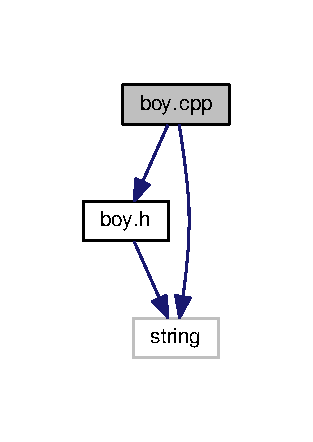
\includegraphics[width=150pt]{boy_8cpp__incl}
\end{center}
\end{figure}

\hypertarget{boy_8h}{}\section{boy.\+h File Reference}
\label{boy_8h}\index{boy.\+h@{boy.\+h}}
{\ttfamily \#include $<$string$>$}\\*
Include dependency graph for boy.\+h\+:
\nopagebreak
\begin{figure}[H]
\begin{center}
\leavevmode
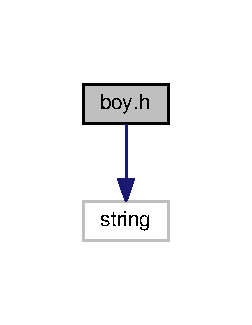
\includegraphics[width=121pt]{boy_8h__incl}
\end{center}
\end{figure}
This graph shows which files directly or indirectly include this file\+:
\nopagebreak
\begin{figure}[H]
\begin{center}
\leavevmode
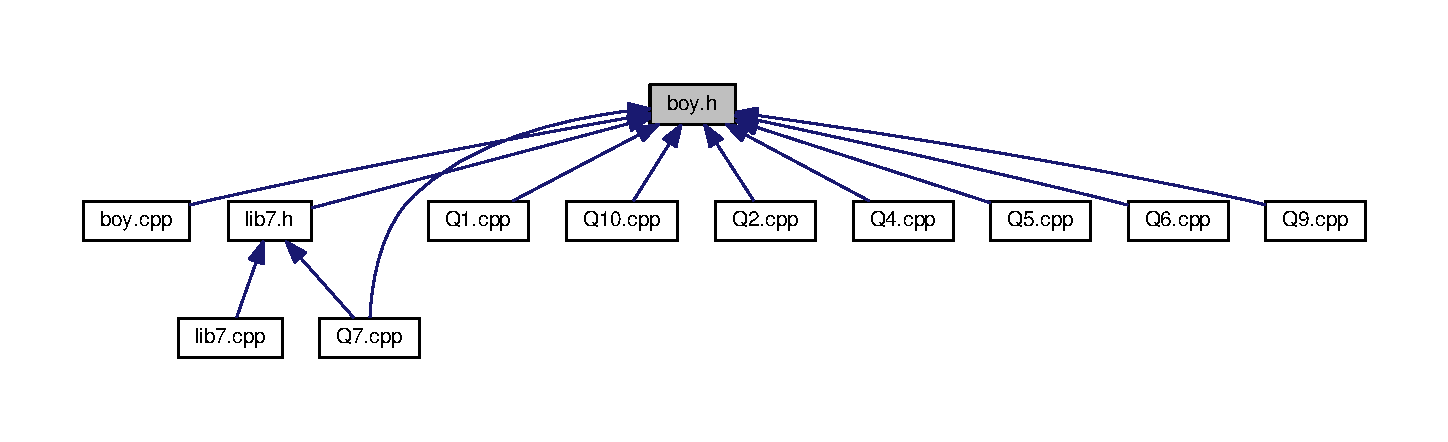
\includegraphics[width=263pt]{boy_8h__dep__incl}
\end{center}
\end{figure}
\subsection*{Classes}
\begin{DoxyCompactItemize}
\item 
class \hyperlink{classBoy}{Boy}
\end{DoxyCompactItemize}

\hypertarget{boyrec_8txt}{}\section{boyrec.\+txt File Reference}
\label{boyrec_8txt}\index{boyrec.\+txt@{boyrec.\+txt}}

\hypertarget{couple_8cpp}{}\section{couple.\+cpp File Reference}
\label{couple_8cpp}\index{couple.\+cpp@{couple.\+cpp}}
{\ttfamily \#include \char`\"{}couple.\+h\char`\"{}}\\*
{\ttfamily \#include $<$string$>$}\\*
{\ttfamily \#include $<$cmath$>$}\\*
Include dependency graph for couple.\+cpp\+:
\nopagebreak
\begin{figure}[H]
\begin{center}
\leavevmode
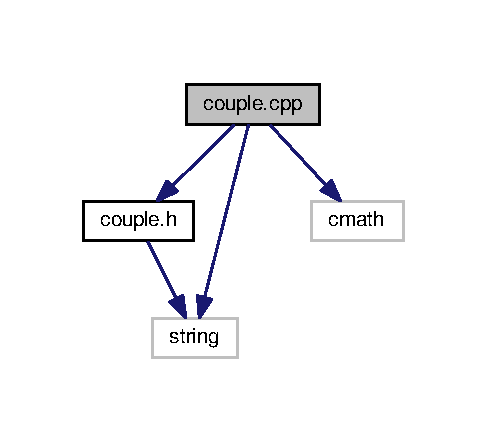
\includegraphics[width=233pt]{couple_8cpp__incl}
\end{center}
\end{figure}

\hypertarget{couple_8h}{}\section{couple.\+h File Reference}
\label{couple_8h}\index{couple.\+h@{couple.\+h}}
{\ttfamily \#include $<$string$>$}\\*
Include dependency graph for couple.\+h\+:
\nopagebreak
\begin{figure}[H]
\begin{center}
\leavevmode
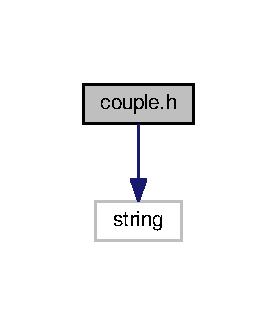
\includegraphics[width=133pt]{couple_8h__incl}
\end{center}
\end{figure}
This graph shows which files directly or indirectly include this file\+:
\nopagebreak
\begin{figure}[H]
\begin{center}
\leavevmode
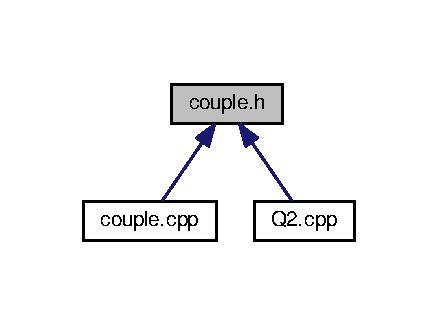
\includegraphics[width=350pt]{couple_8h__dep__incl}
\end{center}
\end{figure}
\subsection*{Classes}
\begin{DoxyCompactItemize}
\item 
class \hyperlink{classcouple}{couple}
\end{DoxyCompactItemize}

\hypertarget{gift_8cpp}{}\section{gift.\+cpp File Reference}
\label{gift_8cpp}\index{gift.\+cpp@{gift.\+cpp}}
{\ttfamily \#include \char`\"{}gift.\+h\char`\"{}}\\*
{\ttfamily \#include $<$string$>$}\\*
Include dependency graph for gift.\+cpp\+:
\nopagebreak
\begin{figure}[H]
\begin{center}
\leavevmode
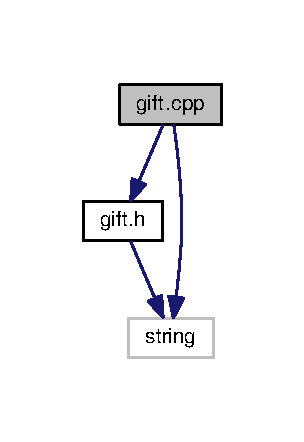
\includegraphics[width=146pt]{gift_8cpp__incl}
\end{center}
\end{figure}

\hypertarget{gift_8h}{}\section{gift.\+h File Reference}
\label{gift_8h}\index{gift.\+h@{gift.\+h}}
{\ttfamily \#include $<$string$>$}\\*
Include dependency graph for gift.\+h\+:
\nopagebreak
\begin{figure}[H]
\begin{center}
\leavevmode
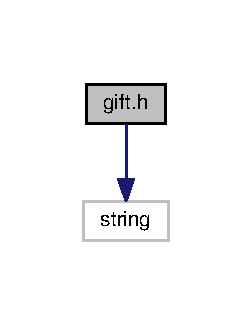
\includegraphics[width=121pt]{gift_8h__incl}
\end{center}
\end{figure}
This graph shows which files directly or indirectly include this file\+:
\nopagebreak
\begin{figure}[H]
\begin{center}
\leavevmode
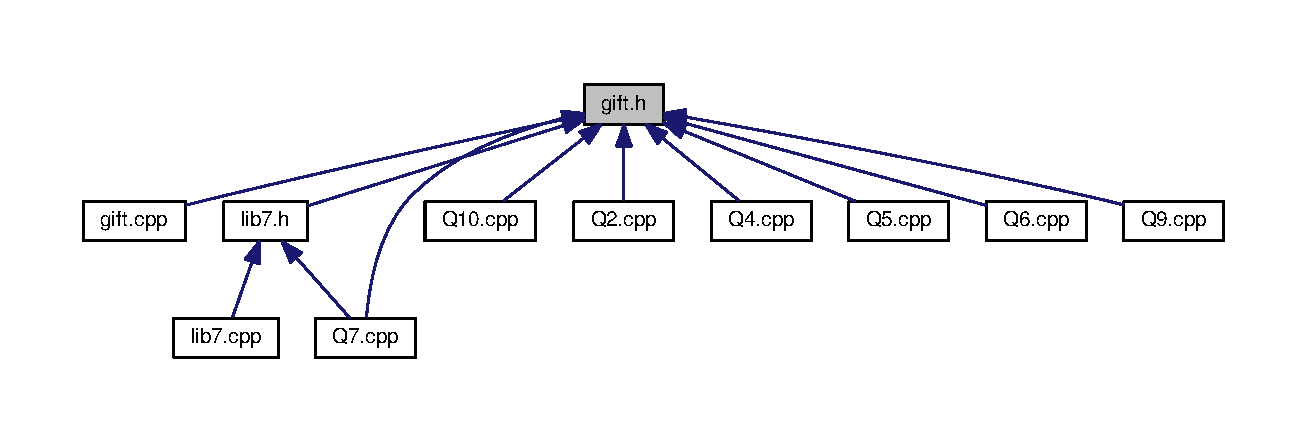
\includegraphics[width=195pt]{gift_8h__dep__incl}
\end{center}
\end{figure}
\subsection*{Classes}
\begin{DoxyCompactItemize}
\item 
class \hyperlink{classGift}{Gift}
\end{DoxyCompactItemize}

\hypertarget{gifts_8txt}{}\section{gifts.\+txt File Reference}
\label{gifts_8txt}\index{gifts.\+txt@{gifts.\+txt}}

\hypertarget{giftslog_8txt}{}\section{giftslog.\+txt File Reference}
\label{giftslog_8txt}\index{giftslog.\+txt@{giftslog.\+txt}}

\hypertarget{girl_8cpp}{}\section{girl.\+cpp File Reference}
\label{girl_8cpp}\index{girl.\+cpp@{girl.\+cpp}}
{\ttfamily \#include \char`\"{}girl.\+h\char`\"{}}\\*
{\ttfamily \#include $<$string$>$}\\*
Include dependency graph for girl.\+cpp\+:
\nopagebreak
\begin{figure}[H]
\begin{center}
\leavevmode
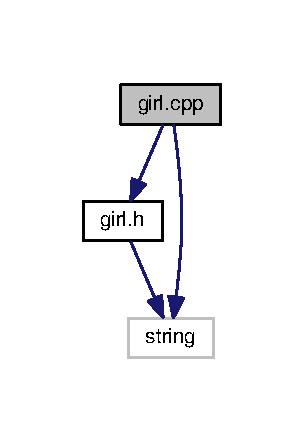
\includegraphics[width=146pt]{girl_8cpp__incl}
\end{center}
\end{figure}

\hypertarget{girl_8h}{}\section{girl.\+h File Reference}
\label{girl_8h}\index{girl.\+h@{girl.\+h}}
{\ttfamily \#include $<$string$>$}\\*
Include dependency graph for girl.\+h\+:
\nopagebreak
\begin{figure}[H]
\begin{center}
\leavevmode
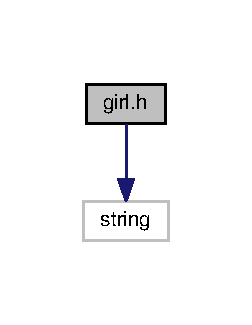
\includegraphics[width=121pt]{girl_8h__incl}
\end{center}
\end{figure}
This graph shows which files directly or indirectly include this file\+:
\nopagebreak
\begin{figure}[H]
\begin{center}
\leavevmode
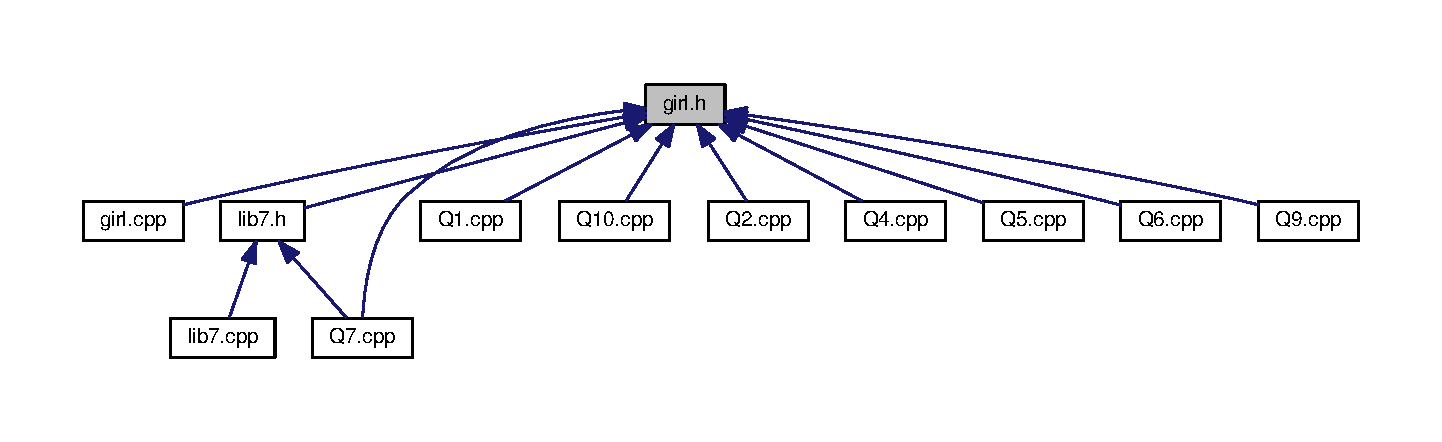
\includegraphics[width=350pt]{girl_8h__dep__incl}
\end{center}
\end{figure}
\subsection*{Classes}
\begin{DoxyCompactItemize}
\item 
class \hyperlink{classGirl}{Girl}
\end{DoxyCompactItemize}

\hypertarget{girlrec_8txt}{}\section{girlrec.\+txt File Reference}
\label{girlrec_8txt}\index{girlrec.\+txt@{girlrec.\+txt}}

\hypertarget{output_8txt}{}\section{output.\+txt File Reference}
\label{output_8txt}\index{output.\+txt@{output.\+txt}}

\hypertarget{Q1_8cpp}{}\section{Q1.\+cpp File Reference}
\label{Q1_8cpp}\index{Q1.\+cpp@{Q1.\+cpp}}
{\ttfamily \#include $<$iostream$>$}\\*
{\ttfamily \#include $<$fstream$>$}\\*
{\ttfamily \#include $<$string$>$}\\*
{\ttfamily \#include \char`\"{}boy.\+h\char`\"{}}\\*
{\ttfamily \#include \char`\"{}girl.\+h\char`\"{}}\\*
Include dependency graph for Q1.\+cpp\+:
\nopagebreak
\begin{figure}[H]
\begin{center}
\leavevmode
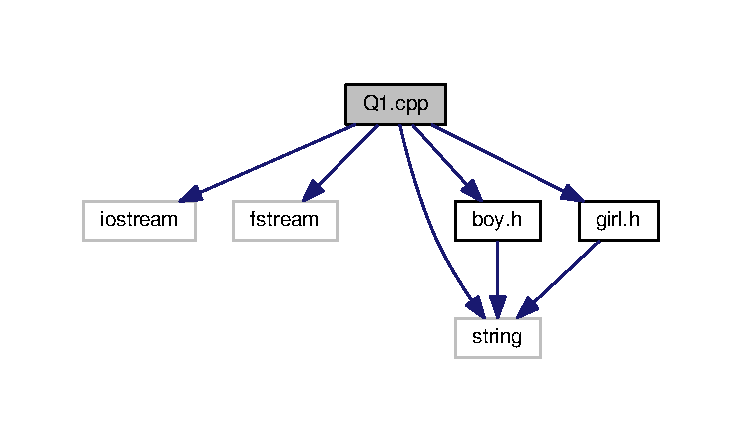
\includegraphics[width=350pt]{Q1_8cpp__incl}
\end{center}
\end{figure}
\subsection*{Functions}
\begin{DoxyCompactItemize}
\item 
int \hyperlink{Q1_8cpp_ae66f6b31b5ad750f1fe042a706a4e3d4}{main} ()
\end{DoxyCompactItemize}


\subsection{Function Documentation}
\index{Q1.\+cpp@{Q1.\+cpp}!main@{main}}
\index{main@{main}!Q1.\+cpp@{Q1.\+cpp}}
\subsubsection[{\texorpdfstring{main()}{main()}}]{\setlength{\rightskip}{0pt plus 5cm}int main (
\begin{DoxyParamCaption}
{}
\end{DoxyParamCaption}
)}\hypertarget{Q1_8cpp_ae66f6b31b5ad750f1fe042a706a4e3d4}{}\label{Q1_8cpp_ae66f6b31b5ad750f1fe042a706a4e3d4}
$<$ Read boys data

$<$ Make Couples 
\begin{DoxyCode}
10 \{
11     ifstream boyPtr(\textcolor{stringliteral}{"boyrec.txt"}, ios::in);
12     ifstream girlPtr(\textcolor{stringliteral}{"girlrec.txt"}, ios::in);
13     ofstream opPtr(\textcolor{stringliteral}{"output.txt"}, ios::out);
14     \textcolor{keywordtype}{int} \hyperlink{lib7_8h_aeee5e31bf47987f4c471a1649ec9e43f}{noBoys} = 7,\hyperlink{lib7_8h_afbf77341ebcfec44fd5ed146e13668bf}{noGirls} = 4;
15     \hyperlink{classBoy}{Boy} boy[\hyperlink{lib7_8h_aeee5e31bf47987f4c471a1649ec9e43f}{noBoys}];
16     \hyperlink{classGirl}{Girl} girl[\hyperlink{lib7_8h_afbf77341ebcfec44fd5ed146e13668bf}{noGirls}];
17     \textcolor{keywordtype}{int} maint, budget,intelli,attr,i;
18     \textcolor{keywordtype}{string} name,girlName,boyName,type;
19     
21     \textcolor{keywordflow}{for}( i = 0; i < \hyperlink{lib7_8h_aeee5e31bf47987f4c471a1649ec9e43f}{noBoys}; i++) \{
22         boyPtr >> name >> type >> attr >> intelli >> budget ;
23         boy[i].\hyperlink{classBoy_aa6d16a472a01b4e7da0817fe94d9a2bd}{init}(name,type,attr,intelli,budget);
24     \}
25 
27     \textcolor{keywordflow}{for}( i = 0; i < \hyperlink{lib7_8h_afbf77341ebcfec44fd5ed146e13668bf}{noGirls}; i++) \{
28         girlPtr >> name >> type >> attr >> intelli >> maint ;
29         girl[i].\hyperlink{classGirl_aba849734c908a23bde2e5bd9c335c450}{init}(name,type,attr,intelli,budget);
30     \}
31 
32     \textcolor{keywordtype}{int} j = 0,k = 0;
34     \textcolor{keywordflow}{for}( i = 0; i < \hyperlink{lib7_8h_afbf77341ebcfec44fd5ed146e13668bf}{noGirls}; i++) \{
35         maint = girl[i].\hyperlink{classGirl_ac23543169a5e339a3c93fbd8aeb977ca}{getMaint}();
36         girlName = girl[i].\hyperlink{classGirl_a27a705fb94b92dfd6929d0bf4bcaf5e1}{getName}();
37         \textcolor{keywordflow}{for}( j = k; j < \hyperlink{lib7_8h_aeee5e31bf47987f4c471a1649ec9e43f}{noBoys}; j++) \{
38             budget = boy[j].\hyperlink{classBoy_a05c48b12091ebcad44ba86ba88514ac5}{getBudget}();
39             boyName = boy[j].\hyperlink{classBoy_acf59fd0074a6ea3413751a95b2970303}{getName}();
40             \textcolor{keywordflow}{if}(maint < budget && !(girl[i].getStatus() ) && !(boy[j].getStatus() ) ) \{
41                     opPtr << girlName << \textcolor{stringliteral}{"        "} << boyName << endl;
42                     girl[i].\hyperlink{classGirl_ac4e040efdf40d12044bda1b647e0d2da}{changeStatus}();
43                     boy[j].\hyperlink{classBoy_a2a8cc82d9332c07eb475198e46028d52}{changeStatus}();
44                     k++;
45                     \textcolor{keywordflow}{break};
46             \} \textcolor{keywordflow}{else} \{
47                 j--;
48             \}
49         \}
50     \}
51 \}
\end{DoxyCode}

\hypertarget{Q2_8cpp}{}\section{Q2.\+cpp File Reference}
\label{Q2_8cpp}\index{Q2.\+cpp@{Q2.\+cpp}}
{\ttfamily \#include $<$iostream$>$}\\*
{\ttfamily \#include $<$fstream$>$}\\*
{\ttfamily \#include $<$string$>$}\\*
{\ttfamily \#include \char`\"{}boy.\+h\char`\"{}}\\*
{\ttfamily \#include \char`\"{}girl.\+h\char`\"{}}\\*
{\ttfamily \#include \char`\"{}couple.\+h\char`\"{}}\\*
{\ttfamily \#include \char`\"{}gift.\+h\char`\"{}}\\*
{\ttfamily \#include $<$cmath$>$}\\*
Include dependency graph for Q2.\+cpp\+:
\nopagebreak
\begin{figure}[H]
\begin{center}
\leavevmode
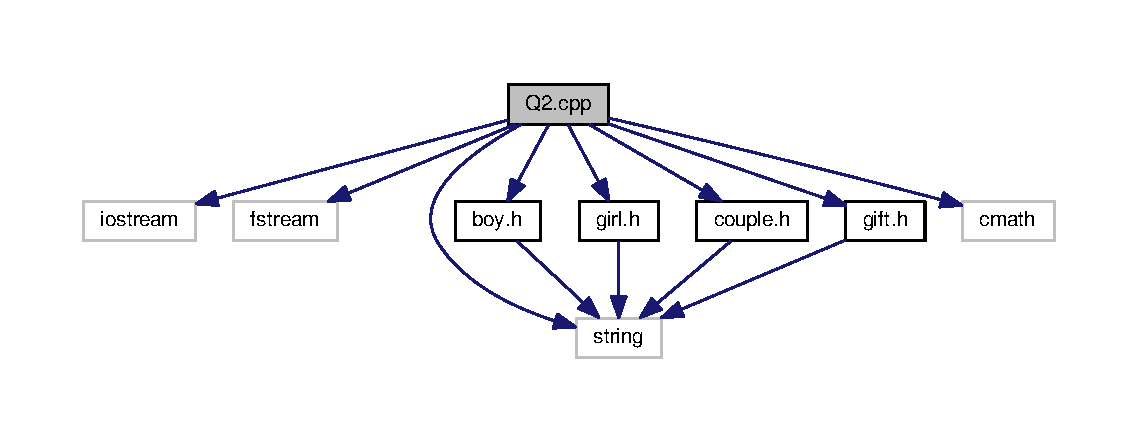
\includegraphics[width=350pt]{Q2_8cpp__incl}
\end{center}
\end{figure}
\subsection*{Functions}
\begin{DoxyCompactItemize}
\item 
void \hyperlink{Q2_8cpp_a5a408068bacb1c7add72673eb9d96bbc}{swap\+Couple} (\hyperlink{classcouple}{couple} \&a, \hyperlink{classcouple}{couple} \&b)
\item 
void \hyperlink{Q2_8cpp_ac5c65f5b5ec33f7b8ab8012de336fdb7}{swapC} (\hyperlink{classcouple}{couple} \&a, \hyperlink{classcouple}{couple} \&b)
\item 
int \hyperlink{Q2_8cpp_ae66f6b31b5ad750f1fe042a706a4e3d4}{main} ()
\end{DoxyCompactItemize}


\subsection{Function Documentation}
\index{Q2.\+cpp@{Q2.\+cpp}!main@{main}}
\index{main@{main}!Q2.\+cpp@{Q2.\+cpp}}
\subsubsection[{\texorpdfstring{main()}{main()}}]{\setlength{\rightskip}{0pt plus 5cm}int main (
\begin{DoxyParamCaption}
{}
\end{DoxyParamCaption}
)}\hypertarget{Q2_8cpp_ae66f6b31b5ad750f1fe042a706a4e3d4}{}\label{Q2_8cpp_ae66f6b31b5ad750f1fe042a706a4e3d4}
$<$ Read boys data

$<$ Read the gifts

$<$ Sort couples according to their happiness

$<$ Print sorted couple in a file \index{Q2.\+cpp@{Q2.\+cpp}!swapC@{swapC}}
\index{swapC@{swapC}!Q2.\+cpp@{Q2.\+cpp}}
\subsubsection[{\texorpdfstring{swap\+C(couple \&a, couple \&b)}{swapC(couple &a, couple &b)}}]{\setlength{\rightskip}{0pt plus 5cm}void swapC (
\begin{DoxyParamCaption}
\item[{{\bf couple} \&}]{a, }
\item[{{\bf couple} \&}]{b}
\end{DoxyParamCaption}
)}\hypertarget{Q2_8cpp_ac5c65f5b5ec33f7b8ab8012de336fdb7}{}\label{Q2_8cpp_ac5c65f5b5ec33f7b8ab8012de336fdb7}
\index{Q2.\+cpp@{Q2.\+cpp}!swap\+Couple@{swap\+Couple}}
\index{swap\+Couple@{swap\+Couple}!Q2.\+cpp@{Q2.\+cpp}}
\subsubsection[{\texorpdfstring{swap\+Couple(couple \&a, couple \&b)}{swapCouple(couple &a, couple &b)}}]{\setlength{\rightskip}{0pt plus 5cm}void swap\+Couple (
\begin{DoxyParamCaption}
\item[{{\bf couple} \&}]{a, }
\item[{{\bf couple} \&}]{b}
\end{DoxyParamCaption}
)}\hypertarget{Q2_8cpp_a5a408068bacb1c7add72673eb9d96bbc}{}\label{Q2_8cpp_a5a408068bacb1c7add72673eb9d96bbc}

\hypertarget{sortedCompatibility_8txt}{}\section{sorted\+Compatibility.\+txt File Reference}
\label{sortedCompatibility_8txt}\index{sorted\+Compatibility.\+txt@{sorted\+Compatibility.\+txt}}

\hypertarget{sortedHappiness_8txt}{}\section{sorted\+Happiness.\+txt File Reference}
\label{sortedHappiness_8txt}\index{sorted\+Happiness.\+txt@{sorted\+Happiness.\+txt}}

%--- End generated contents ---

% Index
\backmatter
\newpage
\phantomsection
\clearemptydoublepage
\addcontentsline{toc}{chapter}{Index}
\printindex

\end{document}
